%!TEX TS-program = xelatex
%!TEX encoding = UTF-8 Unicode
% Awesome CV LaTeX Template for CV/Resume
%
% This template has been downloaded from:
% https://github.com/posquit0/Awesome-CV
%
% Author:
% Claud D. Park <posquit0.bj@gmail.com>
% http://www.posquit0.com
%
% Template license:
% CC BY-SA 4.0 (https://creativecommons.org/licenses/by-sa/4.0/)
%


%-------------------------------------------------------------------------------
% CONFIGURATIONS
%-------------------------------------------------------------------------------
% A4 paper size by default, use 'letterpaper' for US letter
\documentclass[11pt, a4paper]{awesome-cv}
% Configure page margins with geometry
\geometry{left=1.4cm, top=.8cm, right=1.4cm, bottom=1.8cm, footskip=.5cm}

% Specify the location of the included fonts
\fontdir[fonts/]

% Color for highlights
% Awesome Colors: awesome-emerald, awesome-skyblue, awesome-red, awesome-pink, awesome-orange
%                 awesome-nephritis, awesome-concrete, awesome-darknight
\colorlet{awesome}{awesome-red}
% Uncomment if you would like to specify your own color
% \definecolor{awesome}{HTML}{CA63A8}

% Colors for text
% Uncomment if you would like to specify your own color
% \definecolor{darktext}{HTML}{414141}
% \definecolor{text}{HTML}{333333}
% \definecolor{graytext}{HTML}{5D5D5D}
% \definecolor{lighttext}{HTML}{999999}

% Set false if you don't want to highlight section with awesome color
\setbool{acvSectionColorHighlight}{true}

% If you would like to change the social information separator from a pipe (|) to something else
\renewcommand{\acvHeaderSocialSep}{\quad\textbar\quad}


%-------------------------------------------------------------------------------
%	PERSONAL INFORMATION
%	Comment any of the lines below if they are not required
%-------------------------------------------------------------------------------
% Available options: circle|rectangle,edge/noedge,left/right
% \photo{profile.png}
\name{闫}{冰洁}
\position{联邦学习{\enskip\cdotp\enskip}机器学习{\enskip\cdotp\enskip}大数据}
\address{中国·海南省·海口市·美兰区人民大道58号·海南大学}

\mobile{(+86) 156-6667-6912}
\email{bj.yan@ieee.org}
\homepage{bj-yan.top}
\github{beiyuouo}
\googlescholar{DVsgN1sAAAAJ}{B. Yan}
\orcid{0000-0002-8810-9689}{0000-0002-8810-9689}
% \linkedin{beiyuouo}
% \gitlab{gitlab-id}
% \stackoverflow{SO-id}{SO-name}
% \twitter{@twit}
% \skype{skype-id}
% \reddit{reddit-id}
% \extrainfo{extra informations}

\quote{“Nothing is impossible.”}


%-------------------------------------------------------------------------------
\begin{document}

% Print the header with above personal informations
% Give optional argument to change alignment(C: center, L: left, R: right)
\makecvheader

% Print the footer with 3 arguments(<left>, <center>, <right>)
% Leave any of these blank if they are not needed
\makecvfooter
  {\today}
  {Bingjie Yan~~~·~~~Curriculum Vitae}
  {\thepage}


%-------------------------------------------------------------------------------
%	CV/RESUME CONTENT
%	Each section is imported separately, open each file in turn to modify content
%-------------------------------------------------------------------------------
%-------------------------------------------------------------------------------
%        SECTION TITLE
%-------------------------------------------------------------------------------
\cvsection{教育经历}


%-------------------------------------------------------------------------------
%        CONTENT
%-------------------------------------------------------------------------------
\begin{cventries}

%---------------------------------------------------------
\cventry
{硕士{\enskip\cdotp\enskip}计算机科学} % Degree
{中国科学院{\enskip\cdotp\enskip}计算技术研究所} % Institution
{中国·北京} % Location
{2022.09 - Exp. 2025.06} % Date(s)
{
    \begin{cvitems} % Description(s) bullet points
        \item {GPA: 87/100 (3.79/4)}
        % \item {荣获海南大学“三好学生”、“志愿服务标兵”、“最具创新精神和实践能力的大学生”、“优秀毕业生”荣誉称号}
        % \item {获得海南大学一等综合奖学金}
    \end{cvitems}
}

\cventry
{本科{\enskip\cdotp\enskip}软件工程大数据方向} % Degree
{海南大学{\enskip\cdotp\enskip}计算机与科学技术学院} % Institution
{中国·海南} % Location
{2018.09 - 2022.06} % Date(s)
{
    \begin{cvitems} % Description(s) bullet points
        \item {GPA: 89.69/100 (3.67/4),排名: 8/179(4\%),CET-4: 539,CET-6: 478}
        \item {荣获海南大学“三好学生”、“志愿服务标兵”、“最具创新精神和实践能力的大学生”、“优秀毕业生”等荣誉称号}
        \item {获得海南大学一等综合奖学金、二等综合奖学金}
    \end{cvitems}
}

%---------------------------------------------------------
\end{cventries}

%-------------------------------------------------------------------------------
%	SECTION TITLE
%-------------------------------------------------------------------------------
\cvsection{论文成果}


%-------------------------------------------------------------------------------
%	CONTENT
%-------------------------------------------------------------------------------
\begin{cventries}
	%---------------------------------------------------------
	\cventry
	{第一作者} % Role
	{FedCM: A Real-time Contribution Measurement Method for Participants in Federated Learning} % Title
	{IJCNN 2021(CCF-C)} % Location
	{2021.7, Oral Presentation.} % Date(s)
	{
		\begin{cvitems} % Description(s)
			\item {提出了一种实时评估和衡量联邦学习中参与各方贡献的方法}
			\item {该方法相较于传统方法对数据质量和数量拥有更强的敏感度}
		\end{cvitems}
	}

	%---------------------------------------------------------
	\cventry
	{第一作者} % Role
	{An Improved Method for the Fitting and Prediction of the Number of COVID-19 Confirmed Cases Based on LSTM} % Title
	{Computers, Materials \& Continua} % Location
	{2020.5} % Date(s)
	{
		\begin{cvitems} % Description(s)
			\item {提出了一种利用LSTM对疫情人数预测的改进方法}
		\end{cvitems}
	}

	%---------------------------------------------------------
	\cventry
	{第一作者} % Role
	{Experiments of Federated Learning for COVID-19 Chest X-ray Images} % Title
	{ICAIS 2021} % Location
	{2021.7} % Date(s)
	{
		\begin{cvitems} % Description(s)
			\item {首次将联邦学习应用于新型冠状病毒医疗影像的识别和分类工作}
			\item {利用Grad-CAM++方法对卷积层进行解释和可视化}
		\end{cvitems}
	}

	%---------------------------------------------------------
\end{cventries}

%-------------------------------------------------------------------------------
%	SECTION TITLE
%-------------------------------------------------------------------------------
\cvsection{Internships}


%-------------------------------------------------------------------------------
%	CONTENT
%-------------------------------------------------------------------------------

%\cvsubsection{Innovative business practices \& Competition}

\begin{cventries}
%---------------------------------------------------------
\cventry
{Object detection and medical application in Federated Learning} % Job title
{Research Intern @ FedML} % Organization
{Remote} % Location
{2022.06 - 2022.08} % Date(s)
{
    \begin{cvitems}
        \item {Research on object detection and medical application in Federated Learning with MLDevOps.} % TODO: more details
    \end{cvitems}
}
\end{cventries}

\cvsection{Project Experiences}

\begin{cventries}
%---------------------------------------------------------
\cventry
{Subject with Aier Eye Hospital} % Job titl
{Federated collaborative platform system for digital ophthalmology} % Organization
{Beijing, China} % Location
{2021.12 - 2023.06} % Date(s)
{
    \begin{cvitems}
        \item {Researching the design of the federated learning platform and system for ophthalmology}
        \item {Implementing asynchronous federated learning methods on the platform for medical applications.}
    \end{cvitems}
}

%---------------------------------------------------------
% \cventry
% {Research and demonstration of key technologies for federated collaborative modeling of cross-domain trusted fusion.} % Job title
% {Subject with China Unicom Research Institute} % Organization
% {Beijing, China} % Location
% {2022.10 - 2023.10} % Date(s)
% {
%     \begin{cvitems}
%         \item {Research on Federated Learning in digital ophthalmology.}
%     \end{cvitems}
% }

%---------------------------------------------------------
% \cventry
% {Host} % Job title
% {Smart Image: Medical Image Recognition System based on Federated Learning} % Organization
% {Hainan, China} % Location
% {2020.03 - PRESENT} % Date(s)
% {
% 	\begin{minipage}[b]{0.25\linewidth}
% 		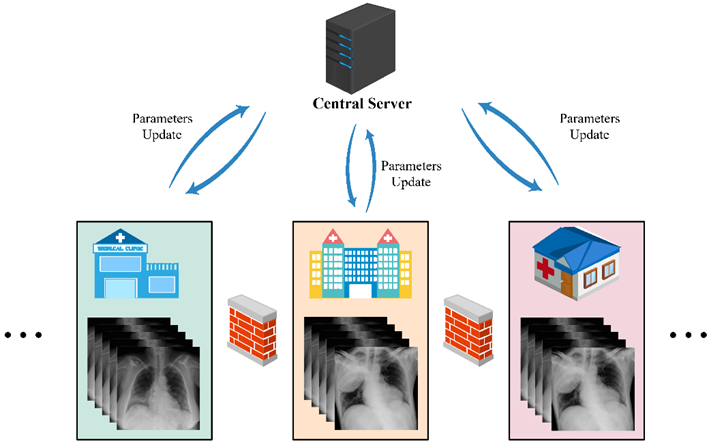
\includegraphics[height=8\baselineskip]{figure/fedcov.png}
% 	\end{minipage}
% 	\hfill
% 	\begin{minipage}[b]{0.7\linewidth}
% 		% 我们设计了一款基于联邦学习的医疗影像识别软件,可以在保护患者数据隐私的前提下进行多方联合。在数据方面,我们汇总了网上的多个公开数据集,并用Pydicom将dicom文件转换成图片形式用于模型识别。在模型方面,我们将包括ResNet、COVID-Net在内的4个模型进行模型融合,增强系统稳定性和泛化能力。同时,我们用GradCAM++对卷积层进行可视化,用于标记病灶位点,最后能够自动化生成医学报告。另外,在多方贡献衡量方面我们提出了FedCM贡献评估算法。
% 		We designed a medical image recognition software based on federated learning that allows for multi-party federation while protecting the privacy of patient data. In the aspect of data, we aggregate several published datasets on the Internet. In terms of models, we fused four models including ResNet and COVID-Net for model fusion to enhance system stability and generalization capability. We use GradCAM++ to visualize the convolutional layers for annotating lesion sites, and finally the software can generate medical reports automatically. In addition, we propose the FedCM contribution evaluation algorithm in the multiparty contribution measurement. \textcolor{awesome-red}{\href{https://github.com/beiyuouo/paddle-fl-gui}{[Code]}}
% 	\end{minipage}
% }

%---------------------------------------------------------
% \cventry
% {Participate} % Job title
% {5G Road Patrol Car} % Organization
% {Hainan, China} % Location
% {2020.05 - PRESENT} % Date(s)
% {
% 	\begin{minipage}[b]{0.25\linewidth}
% 		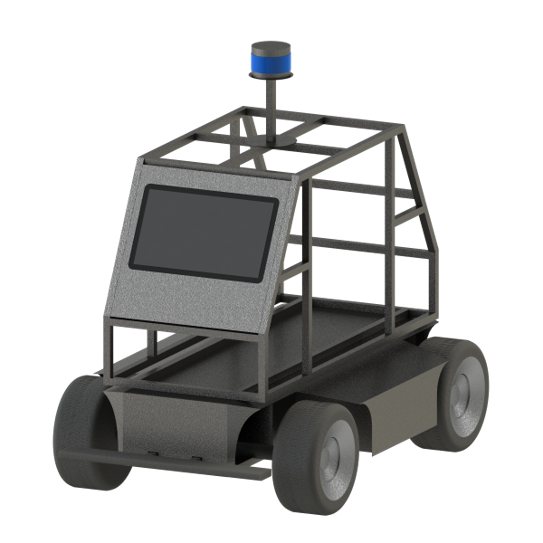
\includegraphics[height=8\baselineskip]{figure/car.png}
% 	\end{minipage}
% 	\hfill
% 	\begin{minipage}[b]{0.7\linewidth}
% 		% 我们设计了一款基于5G和多传感器融合用于城市巡逻的无人路检机器人,主要功能有基于多传感器融合的道路裂缝、坑洼等缺陷检测并进行云端上报,和违停检测。在建图和定位方面,我们基于LeGO-LOAM进行调整和改进。在道路检测方面,我们基于Yolov5训练了自己的模型,F1-score达到了0.68
% 		We designed an unmanned road inspection robot based on 5G and multi-sensor fusion for city patrol. The main functions are multi-sensor fusion-based detection of road cracks, potholes and other defects and reporting them to the cloud, and parking violation detection. For mapping and localization, we adapt and improve the algorithm based on LeGO-LOAM. For road detection, we have trained our own model based on Yolov5, and the F1-score reached 0.68.
% 	\end{minipage}
% }

%---------------------------------------------------------
% \cventry
% {Participate} % Job title
% {ROV technology-based underwater sightseeing robot.} % Organization
% {China} % Location
% {2020.05 - PRESENT} % Date(s)
% {
% 	This is a national student innovation and entrepreneurship project. We use underwater ROV for image collection and transmission. After defogging, we perform stitching of video frame sequences to achieve panoramic landscape viewing.
% }

%---------------------------------------------------------
%\end{cventries}

%\cvsubsection{Open Source Project}

%\begin{cventries}
%---------------------------------------------------------
%	\cventry
%	{Owner} % Job title
%	{FedMedical:PaddleFL-based Federated Learning Medical Image Recognition Software} % Organization
%	{\href{https://github.com/beiyuouo/paddle-fl-gui}{\color{awesome-red}{[GitHub link]}}} % Location
%	{2020.11 - PRESENT} % Date(s)
%	{
%		\begin{cvitems} % Description(s) of tasks/responsibilities
%			\item {Distributed Deployment and Federated Learning Simultaneous Training with PaddleFL Framework.}
%		\end{cvitems}
%	}

%---------------------------------------------------------
% \cventry
% {Owner} % Job title
% {Mid-air Draw: Gesture Recognition and Tracking based on YOLOv5} % Organization
% {Hainan, China} % Location
% {2020.09 - PRESENT} % Date(s)
% {
% 	We label the data ourselves and use YOLOv5 for gesture recognition and finger key point recognition. It is able to interact with PPT and other software to achieve the function of mid-air drawing. \textcolor{awesome-red}{\href{https://github.com/beiyuouo/mid-air-draw}{[Code]}} \textcolor{awesome-red}{\href{https://www.bilibili.com/video/BV15V411a7WB/}{[Video]}}
% }

	
%---------------------------------------------------------
\end{cventries}


%-------------------------------------------------------------------------------
%    SECTION TITLE
%-------------------------------------------------------------------------------
\cvsection{荣誉 \& 奖项}


%-------------------------------------------------------------------------------
%    SUBSECTION TITLE
%-------------------------------------------------------------------------------
\cvsubsection{国际}


%-------------------------------------------------------------------------------
%    CONTENT
%-------------------------------------------------------------------------------
\begin{cvhonors}

%---------------------------------------------------------
  \cvhonor
    {银牌} % Award
    {亚太信息学奥林匹克竞赛} % Event
    {中国·北京} % Location
    {2017} % Date(s)

%---------------------------------------------------------
\end{cvhonors}


%-------------------------------------------------------------------------------
%    SUBSECTION TITLE
%-------------------------------------------------------------------------------
\cvsubsection{国家级}


%-------------------------------------------------------------------------------
%    CONTENT
%-------------------------------------------------------------------------------
\begin{cvhonors}

%---------------------------------------------------------
  \cvhonor
    {一等奖} % Award
    {第三届丝绸之路机器人创意赛} % Event
    {中国·西安} % Location
    {2019} % Date(s)

%---------------------------------------------------------
  \cvhonor
    {二等奖} % Award
    {高教社杯中国大学生数学建模竞赛} % Event
    {中国} % Location
    {2020} % Date(s)
    
%---------------------------------------------------------
    \cvhonor
    {个人二等奖} % Award
    {中国高校计算机大赛-团队程序设计天梯赛} % Event
    {中国} % Location
    {2020} % Date(s)

%---------------------------------------------------------
    \cvhonor
    {二等奖} % Award
    {中国大学生计算机设计大赛} % Event
    {中国} % Location
    {2021} % Date(s)

%---------------------------------------------------------
%    \cvhonor
%    {铜奖} % Award
%    {“挑战杯”大学生创业计划竞赛} % Event
%    {中国} % Location
%    {2020} % Date(s)

%---------------------------------------------------------
    \cvhonor
    {铜奖} % Award
    {“互联网+”大学生创新创业大赛} % Event
    {中国} % Location
    {2020} % Date(s)

%---------------------------------------------------------
    \cvhonor
    {三等奖} % Award
    {中国高校计算机大赛-人工智能创意赛} % Event
    {中国·杭州} % Location
    {2020} % Date(s)

%---------------------------------------------------------
\end{cvhonors}

\cvsubsection{省级}


%-------------------------------------------------------------------------------
%    CONTENT
%-------------------------------------------------------------------------------
\begin{cvhonors}
    
    %---------------------------------------------------------
    \cvhonor
    {特等奖} % Award
    {中国高校计算机大赛-团队程序设计天梯赛} % Event
    {中国·海南} % Location
    {2020} % Date(s)
    
        
    %---------------------------------------------------------
    \cvhonor
    {金奖\&银奖} % Award
    {第六、七届中国国际“互联网+”大学生创新创业竞赛海南赛区} % Event
    {中国·海南} % Location
    {2020,2021} % Date(s)
    
    %---------------------------------------------------------
    %\cvhonor
    %{一等奖} % Award
    %{中国高校计算机设计大赛-海南赛区} % Event
    %{中国·海南} % Location
    %{2021} % Date(s)
    
    %---------------------------------------------------------
    %\cvhonor
    %{二等奖} % Award
    %{中国高校计算机大赛-人工智能创意赛-华南赛区} % Event
    %{中国·海南} % Location
    %{2020} % Date(s)
    
    %---------------------------------------------------------
    \cvhonor
    {三等奖} % Award
    {“挑战杯”中国大学生课外学术竞赛-海南赛区} % Event
    {中国·海南} % Location
    {2021} % Date(s)
    
    %---------------------------------------------------------
\end{cvhonors}

%-------------------------------------------------------------------------------
%	SECTION TITLE
%-------------------------------------------------------------------------------
\cvsection{Skills \& Interests}


%-------------------------------------------------------------------------------
%	CONTENT
%-------------------------------------------------------------------------------
\begin{cvskills}
	
%---------------------------------------------------------
\cvskill
{Language} % Category
{Chinese(Native), English(Fluent, CET-6: 478, CET-4: 539, IELTS: working on!!)} % Skills

%---------------------------------------------------------
\cvskill
{Photography} % Category
{Enjoy the life and capture the moments :)} % Skills

%---------------------------------------------------------
%  \cvskill
%    {Programming languages} % Category
%    {Python, Java, C++} % Skills
%---------------------------------------------------------
	% \cvskill
	% {Machine Learning} % Category
	% {PyTorch, TensorFlow, OpenCV} % Skills
%---------------------------------------------------------
%	\cvskill
%	{Robotics} % Category
%	{ROS Melodic} % Skills
%---------------------------------------------------------
%   \cvskill
%     {Big data} % Category
%     {Hadoop, HBase, Hive, ZooKeeper, Storm, Kafka, Sqoop, Flume} % Skills
%---------------------------------------------------------
%	\cvskill
%	{Front-end} % Category
%	{Springboot, Mybatis, Flask} % Skills

%---------------------------------------------------------
\end{cvskills}

%-------------------------------------------------------------------------------
%    SECTION TITLE
%-------------------------------------------------------------------------------
\cvsection{任职经历}


%-------------------------------------------------------------------------------
%    CONTENT
%-------------------------------------------------------------------------------
\begin{cventries}
%---------------------------------------------------------
    \cventry
    {主席} % Affiliation/role
    {IEEE 海南大学学生分会} % Organization/group
    {中国·海南} % Location
    {2021.03 - 2022.06} % Date(s)
    {
        \begin{cvitems} % Description(s) of experience/contributions/knowledge
            \item{参与前沿学术会议,了解前沿学术动态}
        \end{cvitems}
    }


%---------------------------------------------------------
    \cventry
    {副会长} % Affiliation/role
    {海南大学机器人与人工智能协会} % Organization/group
    {中国·海南} % Location
    {2020.07 - 2022.06} % Date(s)
    {
        \begin{cvitems} % Description(s) of experience/contributions/knowledge
            \item{学习机器学习知识,组织组员参与和筹备相关竞赛和项目,开展机器学习分享会、讲座}
        \end{cvitems}
    }

%---------------------------------------------------------
    % \cventry
    % {新闻宣传部部长} % Affiliation/role
    % {海南大学计算机与网络空间安全学院青年志愿者协会} % Organization/group
    % {中国·海南} % Location
    % {2019.09 - 2020.07} % Date(s)
    % {
    %     \begin{cvitems} % Description(s) of experience/contributions/knowledge
    %     \item {参与各项志愿活动}
    %     \item {提升领导和工作分配能力}
    %     \end{cvitems}
    % }

%---------------------------------------------------------
    % \cventry
    % {副会长} % Affiliation/role
    % {海南大学网络空间安全协会} % Organization/group
    % {中国·海南} % Location
    % {2019.09 - 2020.07} % Date(s)
    % {
    %     \begin{cvitems} % Description(s) of experience/contributions/knowledge
    %         \item{了解网络安全相关知识}
    %         \item{了解和进行协会活动筹备等相关工作}
    %     \end{cvitems}
    % }
%---------------------------------------------------------
\end{cventries}

%%-------------------------------------------------------------------------------
%    SECTION TITLE
%-------------------------------------------------------------------------------
\cvsection{Presentation}


%-------------------------------------------------------------------------------
%    CONTENT
%-------------------------------------------------------------------------------
\begin{cventries}

%---------------------------------------------------------
  \cventry
    {Presenter for <DEFCON 20th : The way to go to Las Vegas>} % Role
    {6th CodeEngn (Reverse Engineering Conference)} % Event
    {Seoul, S.Korea} % Location
    {Jul. 2012} % Date(s)
    {
      \begin{cvitems} % Description(s)
        \item {Introduced CTF(Capture the Flag) hacking competition and advanced techniques and strategy for CTF}
      \end{cvitems}
    }

%---------------------------------------------------------
  \cventry
    {Presenter for <Metasploit 101>} % Role
    {6th Hacking Camp - S.Korea} % Event
    {S.Korea} % Location
    {Sep. 2012} % Date(s)
    {
      \begin{cvitems} % Description(s)
        \item {Introduced basic procedure for penetration testing and how to use Metasploit}
      \end{cvitems}
    }

%---------------------------------------------------------
\end{cventries}

%%-------------------------------------------------------------------------------
%	SECTION TITLE
%-------------------------------------------------------------------------------
\cvsection{Writing}


%-------------------------------------------------------------------------------
%	CONTENT
%-------------------------------------------------------------------------------
\begin{cventries}

%---------------------------------------------------------
  \cventry
    {Founder \& Writer} % Role
    {A Guide for Developers in Start-up} % Title
    {Facebook Page} % Location
    {Jan. 2015 - PRESENT} % Date(s)
    {
      \begin{cvitems} % Description(s)
        \item {Drafted daily news for developers in Korea about IT technologies, issues about start-up.}
      \end{cvitems}
    }

%---------------------------------------------------------
\end{cventries}

%%-------------------------------------------------------------------------------
%	SECTION TITLE
%-------------------------------------------------------------------------------
\cvsection{Program Committees}


%-------------------------------------------------------------------------------
%	CONTENT
%-------------------------------------------------------------------------------
\begin{cvhonors}

%---------------------------------------------------------
  \cvhonor
    {Problem Writer} % Position
    {2016 CODEGATE Hacking Competition World Final} % Committee
    {S.Korea} % Location
    {2016} % Date(s)

%---------------------------------------------------------
  \cvhonor
    {Organizer \& Co-director} % Position
    {1st POSTECH Hackathon} % Committee
    {S.Korea} % Location
    {2013} % Date(s)

%---------------------------------------------------------
  \cvhonor
    {Staff} % Position
    {7th Hacking Camp} % Committee
    {S.Korea} % Location
    {2012} % Date(s)

%---------------------------------------------------------
  \cvhonor
    {Problem Writer} % Position
    {1st Hoseo University Teenager Hacking Competition} % Committee
    {S.Korea} % Location
    {2012} % Date(s)

%---------------------------------------------------------
  \cvhonor
    {Staff \& Problem Writer} % Position
    {JFF(Just for Fun) Hacking Competition} % Committee
    {S.Korea} % Location
    {2012} % Date(s)

%---------------------------------------------------------
\end{cvhonors}



%-------------------------------------------------------------------------------
\end{document}
